\section{OpenMP parallelization and execution analysis: Gauss-Seidel}

\subsection{Parallelization}
\justify
In this section we are going to parallelize the Gauus-Seidel algorithm. The parallelization is going to be different since the dependencies are different, as we seen on the first section. In this case, there are dependencies between iterations inside the Gauss function, more specifically with adjacent positions of the matrix \textit{u.}
\justify
We also have to do the same adjustments to the variable sum and diff, with the addition of a new one called unew. The first one is going to be a reduction and the last two are going to be private for each thread.
\justify
In this algorithm we first used the \#pragma omp for ordered construct, which assures the correct execution of nested loops in order. This is needed because we will also be using the depend clause in order to indicate the dependencies between the matrix. First, we use the sink clause to mark the dependencies to previous iterations and then we use the source clause to indicate that the corresponding iteration has finished its work.
\justify
Here you can see the code with all the pragmas:

\begin{lstlisting}
double relax_gauss (double *u, unsigned sizex, unsigned sizey)
{
  double unew, diff, sum=0.0;
  #pragma omp parallel for ordered(2) reduction(+:sum) 
                                    private(diff,unew)
  for (int i=1; i<= sizex-2; i++) {
    for (int j=1; j<= sizey-2; j++) {
      #pragma omp ordered depend (sink:i,j-1) depend (sink:i-1,j)
      unew= 0.25 * ( u[ i*sizey	+ (j-1) ]+  // left
				u[i*sizey + (j+1) ]+  // right
				u[(i-1)*sizey + j ]+  // top
				u[(i+1)*sizey + j]); // bottom
      diff = unew - u[i*sizey+ j];
      sum += diff * diff; 
      u[i*sizey+j]=unew;
      #pragma omp ordered depend (source)
	}
  }
  return sum;
}
\end{lstlisting}

\subsection{Performance evaluation}
\justify
Just looking at the execution time of this version is enough to tell that this version is far from ideal. The sequential code got an execution time of 6.279s and 1402.62 MFlop\/s and the parallel one 95.355s and 92.35 Mflop\/s. This means a decrease of 1418.63\%; a really terrible parallelization. This is due to the overhead given by the dependencies. 
\justify
The execution lasts so long that it isn't viable to show paraver captures or strong plots, but it's easy to imagine how terrible they would be considering the increase of the execution time. We could change the granularity in order to maybe get a better performance, but we decided to try to implement another type of parallelization instead since the first method has already been used in the past lab assignments.

\subsection{New approach}
\justify
In order to parallelize this algorithm we are going to need a really different approach. Instead of using the \#pragma omp for clause we are going to implement a data decomposition similar to the one in Jacobi's algorithm. This means applying a geometric block data decomposition. First, we are going to implement it the same way as in Jacobi's algorithm and see what problem we encounter.
\justify
First, we are going to use the following code:
\begin{lstlisting}
double relax_gauss (double *u, unsigned sizex, unsigned sizey)
{
  double unew, diff, sum=0.0;
  int howmanyx = omp_get_num_threads();
  #pragma omp parallel for ordered(1) reduction(+:sum)  
                                   private(unew) private(diff)
  for (int blockidi = 0; blockidi < howmanyx; ++blockidi) {
    int i_start = lowerb(blockidi, howmanyx, sizex);
    int i_end   = upperb(blockidi, howmanyx, sizex);
    #pragma omp ordered depend(sink:blockidi-1)
    for (int i=max(1, i_start); i<= min(sizex-2, i_end); i++) {
      for (int j=1; j<= sizey-2; j++) {
        unew= 0.25 * ( u[i*sizey + (j-1)]+  // left
			u[i*sizey + (j+1)]+  // right
			u[(i-1)*sizey + j]+  // top
			u[(i+1)*sizey + j]); // bottom
        diff = unew - u[i*sizey+ j];
        sum += diff * diff; 
        u[i*sizey+j]=unew;
      } 
    }
    #pragma omp ordered depend(sink:source)
  }
  return sum;
}
\end{lstlisting}
\justify
With this version, we obtain an execution time of 6.763 and 1302.18 Mflop\/s. This is still a decrease in execution time (7.71\%) but much better than the previous version. The execution is actually like the serial one, since each block has to wait until the previous one has finished to start. The extra time is due to OpenMP overheads.

\justify
Making a simple block decomposition by rows makes us have to wait until all the computation of the previous block has finished until the next one can start. This is caused by the dependencies that are in the borders of adjacent blocks. To improve this, we are also going to create blocks on the "j" dimension.
\justify
In order to define the size of this blocks, the ideal case would be to have a number of threads with a natural root, so we can have \textit{sqrt(omp\_get\_num\_threads())} blocks in each dimension. Since we can't assure that this will be the case, we thought of a different approach. The number of blocks in the "i" dimension will be the integer floor of the square root of the number of threads; and the number of blocks in the "j" will be the floor of the number of threads divided per the square root. Doing this we get the maximum number of blocks evenly distributed among all threads, with each thread doing maximum one block.
\justify
In the following figure you can see an approach of how the data distribution can end. Dependencies are between a block and the one to its left and the one over it.

\begin{figure}[h!]
    \centering
    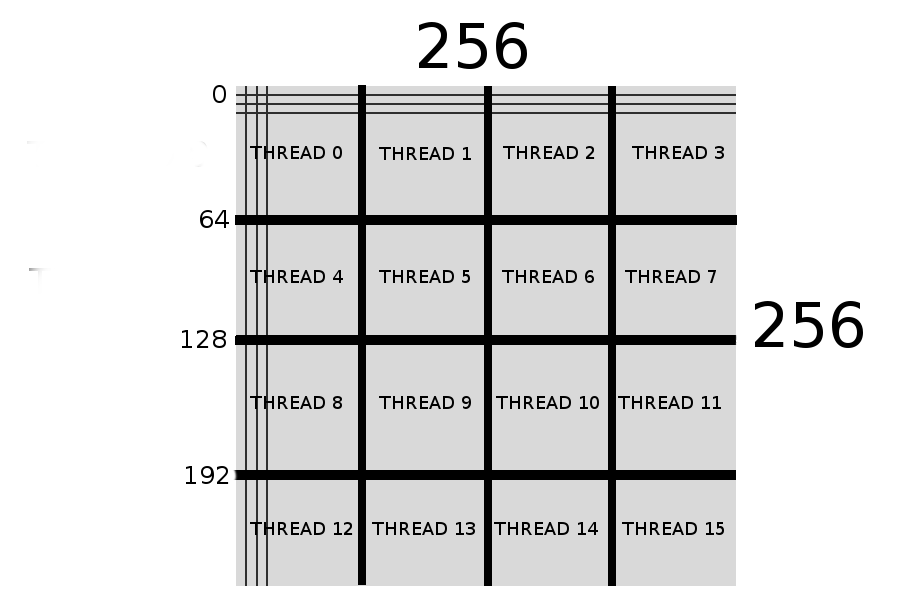
\includegraphics[width=0.80\textwidth]{distribution2.png}
    \caption{Better block distribution}
    \label{fig:distribution2}
\end{figure}


\justify
The code is the following:

\begin{lstlisting}
double relax_gauss (double *u, unsigned sizex, unsigned sizey)
{
  double sum=0.0;
  #pragma omp parallel
  {
  int P = omp_get_num_threads();
  int root = sqrt(P);
  int howmanyi=root;
  int howmanyj=P/root; 
  int id = omp_get_thread_num();
  int id_i = id/howmanyj;
  int id_j = id%howmanyj;
  int i_start = lowerb(id_i, howmanyi, sizex);
  int i_end   = upperb(id_i, howmanyi, sizex);
  int j_start = lowerb(id_j, howmanyj, sizey);
  int j_end   = upperb(id_j, howmanyj, sizey);
  #pragma omp task depend(out:u[i_end*sizey + j_end]) 
                depend(in:u[sizey*(i_start-1)+j_end])
                 depend(in:u[sizey*i_end+j_start-1])
  {
  double tmp = 0.0; 
  for (int i=max(1, i_start); i<= min(sizex-2, i_end); i++) {
    for (int j=max(1, j_start); j<= min(sizey-2, j_end); j++) {
      double unew= 0.25 * ( u[ i*sizey	+ (j-1) ]+  // left
		u[ i*sizey	+ (j+1) ]+  // right
		u[ (i-1)*sizey	+ j     ]+  // top
		u[ (i+1)*sizey	+ j     ]); // bottom
      double diff = unew - u[i*sizey+ j];
      tmp += diff*diff;
      u[i*sizey+j]=unew;
    } 
  }
  #pragma omp atomic
  sum += tmp;
  }
  }
  return sum;
}
\end{lstlisting}

\justify
When trying to evaluate this code, the result wasn't correct and we weren't able to fix it. We also tried the following code, but it didnt work. The result was really close to the sequential one, but not quite. We haven't been able to find what is causing it or another way to write the algorithm.

\begin{lstlisting}
struct abc{
	double sum;
	int done;
};
double relax_gauss (double *u, unsigned sizex, unsigned sizey)
{
  double sum=0.0;
  struct abc thread_vector[omp_get_max_threads()];
  for(int i=0;i<omp_get_max_threads();++i) {
    thread_vector[i].sum = 0.0;
    thread_vector[i].done = 0;
  }	
  #pragma omp parallel
  {
  int P = omp_get_num_threads();
  int root = sqrt(P);
  int howmanyi=root;
  int howmanyj=P/root; 
  int id = omp_get_thread_num();
  int id_i = id/howmanyj;
  int id_j = id%howmanyj;
  int i_start = lowerb(id_i, howmanyi, sizex);
  int i_end   = upperb(id_i, howmanyi, sizex);
  int j_start = lowerb(id_j, howmanyj, sizey);
  int j_end   = upperb(id_j, howmanyj, sizey);
  while((id>howmanyj && thread_vector[id-howmanyj].done==0) || 
                    (id_j>0 && thread_vector[id-1].done==0)){
    __asm__("nop");
  }
  for (int i=max(1, i_start); i<= min(sizex-2, i_end); i++) {
    for (int j=max(1, j_start); j<= min(sizey-2, j_end); j++) {
      double unew= 0.25 * ( u[ i*sizey	+ (j-1) ]+  // left
		u[ i*sizey	+ (j+1) ]+  // right
		u[ (i-1)*sizey	+ j     ]+  // top
		u[ (i+1)*sizey	+ j     ]); // bottom
      double diff = unew - u[i*sizey+ j];
      thread_vector[id].sum += diff*diff;
      u[i*sizey+j]=unew;
    } 
  }
  thread_vector[id].done=1;
  }
  for(int i=0; i<omp_get_max_threads(); ++i) 
    sum+=thread_vector[i].sum;
  return sum;
}
\end{lstlisting}